\chapter{Les gènes et l'ADN}\label{ch:g9:genes-and-dna}

Les \omterm{def:g9:chromosomes:chromosomes}{chromosomes} portent les déterminants --- mais un fil
n'est pas encore un texte. Qu'\emph{est-ce} qu'un
déterminant, le long d'un \omterm{def:g9:chromosomes:chromosomes}{chromosome}~? Et de quoi le fil
est-il fait, pour qu'un \omterm{def:g6:cell-unit-of-life:parts}{noyau} large de quelques millièmes de
millimètre puisse contenir les consignes d'un être humain
entier (\cref{exo:g9:heredity-and-traits:12})~? Deux noms
répondent, et ce sont les plus célèbres de la \omterm{def:g1:living-or-not:living}{biologie}
moderne~: le \omterm{def:g9:genes-and-dna:gene}{gène}, et l'\omterm{def:g9:genes-and-dna:dna}{ADN}.

\section{Les gènes~: les déterminants, situés}

\begin{definition}[Gène et allèles]\label{def:g9:genes-and-dna:gene}
Un \emph{gène}\index{gène} est un déterminant rendu
précis~: un \emph{segment de \omterm{def:g9:chromosomes:chromosomes}{chromosome}} qui porte les
consignes de la part de construction d'un \omterm{def:g9:heredity-and-traits:traits}{caractère} --- un
gène pour la machinerie des groupes sanguins, d'autres pour
les pigments de la couleur des \omterm{def:g1:the-five-senses:sense}{yeux}, des milliers et des
milliers le long des 46 fils, chacun à son adresse fixe. Un
gène peut exister en plusieurs versions --- les
\emph{allèles}\index{allèle}~: les versions A, B et O du
gène des groupes sanguins, les versions brune et bleue du
gène de la couleur des \omterm{def:g1:the-five-senses:sense}{yeux}. Même adresse, orthographe
différente.
\end{definition}

\begin{proposition}[Deux exemplaires, et ce que montrer veut dire]\label{prop:g9:genes-and-dna:twocopies}
Les \omterm{def:g9:chromosomes:chromosomes}{chromosomes} vont par paires
(\cref{prop:g9:chromosomes:counts}) --- tout \omterm{def:g9:genes-and-dna:gene}{gène} existe
donc en \emph{deux exemplaires}, un par partenaire, un de
chaque parent. Les deux exemplaires peuvent être le même
\omterm{def:g9:genes-and-dna:gene}{allèle} ou deux \omterm{def:g9:genes-and-dna:gene}{allèles} différents~; s'ils diffèrent, l'un
peut être \emph{exprimé} et l'autre porté en silence --- et
les mystères de l'album de famille se résolvent en
mécanisme~:
\begin{itemize}
  \item le port sans affichage
        (\cref{ex:g9:heredity-and-traits:skip})~: l'\omterm{def:g9:genes-and-dna:gene}{allèle}
        silencieux voyage sur le second partenaire~;
  \item l'enfant du groupe O né de parents A et B
        (\cref{pb:g9:heredity-and-traits:1})~: chaque
        parent portait O en silence, et la réduction de
        moitié a distribué les deux O ensemble~;
  \item l'enfant aux \omterm{def:g1:the-five-senses:sense}{yeux} bleus de parents aux \omterm{def:g1:the-five-senses:sense}{yeux}
        bruns~: deux bleus silencieux qui se rencontrent
        --- une chance sur quatre, quand chacun des deux parents
        en porte un~: la réduction distribue le bleu de
        chaque parent avec une chance sur deux, et les deux
        distributions sont indépendantes.
\end{itemize}
\end{proposition}
\admitted

\begin{example}[Les groupes sanguins, entièrement mécanisés]\label{ex:g9:genes-and-dna:bloodgroups}
Un \omterm{def:g9:genes-and-dna:gene}{gène}, trois \omterm{def:g9:genes-and-dna:gene}{allèles}, deux exemplaires par personne~: A
avec A ou O montre le groupe A~; B avec B ou O montre B~; A
avec B montre AB (les deux exprimés --- les \omterm{def:g9:genes-and-dna:gene}{allèles} ne sont
pas toujours réductibles au silence)~; O avec O montre O.
Tout le motif du registre des dons --- y compris chaque
«~surprise~» --- est l'arithmétique de distributions à deux
exemplaires.
\end{example}

\section{L'ADN~: la matière dans laquelle le texte est écrit}

\begin{definition}[L'ADN]\label{def:g9:genes-and-dna:dna}
Chimiquement, un \omterm{def:g9:chromosomes:chromosomes}{chromosome} est une molécule d'\emph{ADN}\index{ADN}
unique, immensément longue et enroulée (avec des protéines
d'emballage)~: un double brin --- la fameuse échelle
torsadée --- dont les barreaux sont des paires de quatre
lettres chimiques. \emph{L'ordre des lettres le long du
brin est l'information}~: un \omterm{def:g9:genes-and-dna:gene}{gène} est un tronçon de cette
suite, comme une phrase est un tronçon de page. Quatre
lettres, trois milliards d'exemplaires dans un jeu humain
--- assez de texte pour tout le mode d'emploi d'une
construction, enroulé dans chaque \omterm{def:g6:cell-unit-of-life:parts}{noyau}.
\end{definition}

\begin{example}[La voir soi-même]\label{ex:g9:genes-and-dna:extraction}
L'\omterm{def:g9:genes-and-dna:dna}{ADN} s'extrait à la cuisine~: écrase une banane ou un
oignon, ajoute de l'eau salée et un peu de liquide
vaisselle (les \omterm{def:g6:cell-unit-of-life:parts}{membranes} défaites --- les enveloppes de
\cref{def:g6:cell-unit-of-life:parts} sont sa cible),
filtre, et verse de l'alcool froid par-dessus~: à la limite
des deux couches monte un écheveau de filaments blanchâtres,
que l'on enroule sur un cure-dent. Ces filaments sont de
l'\omterm{def:g9:genes-and-dna:dna}{ADN} --- la molécule même de ce chapitre, en vrais
centimètres.
\end{example}

\begin{omfigure}
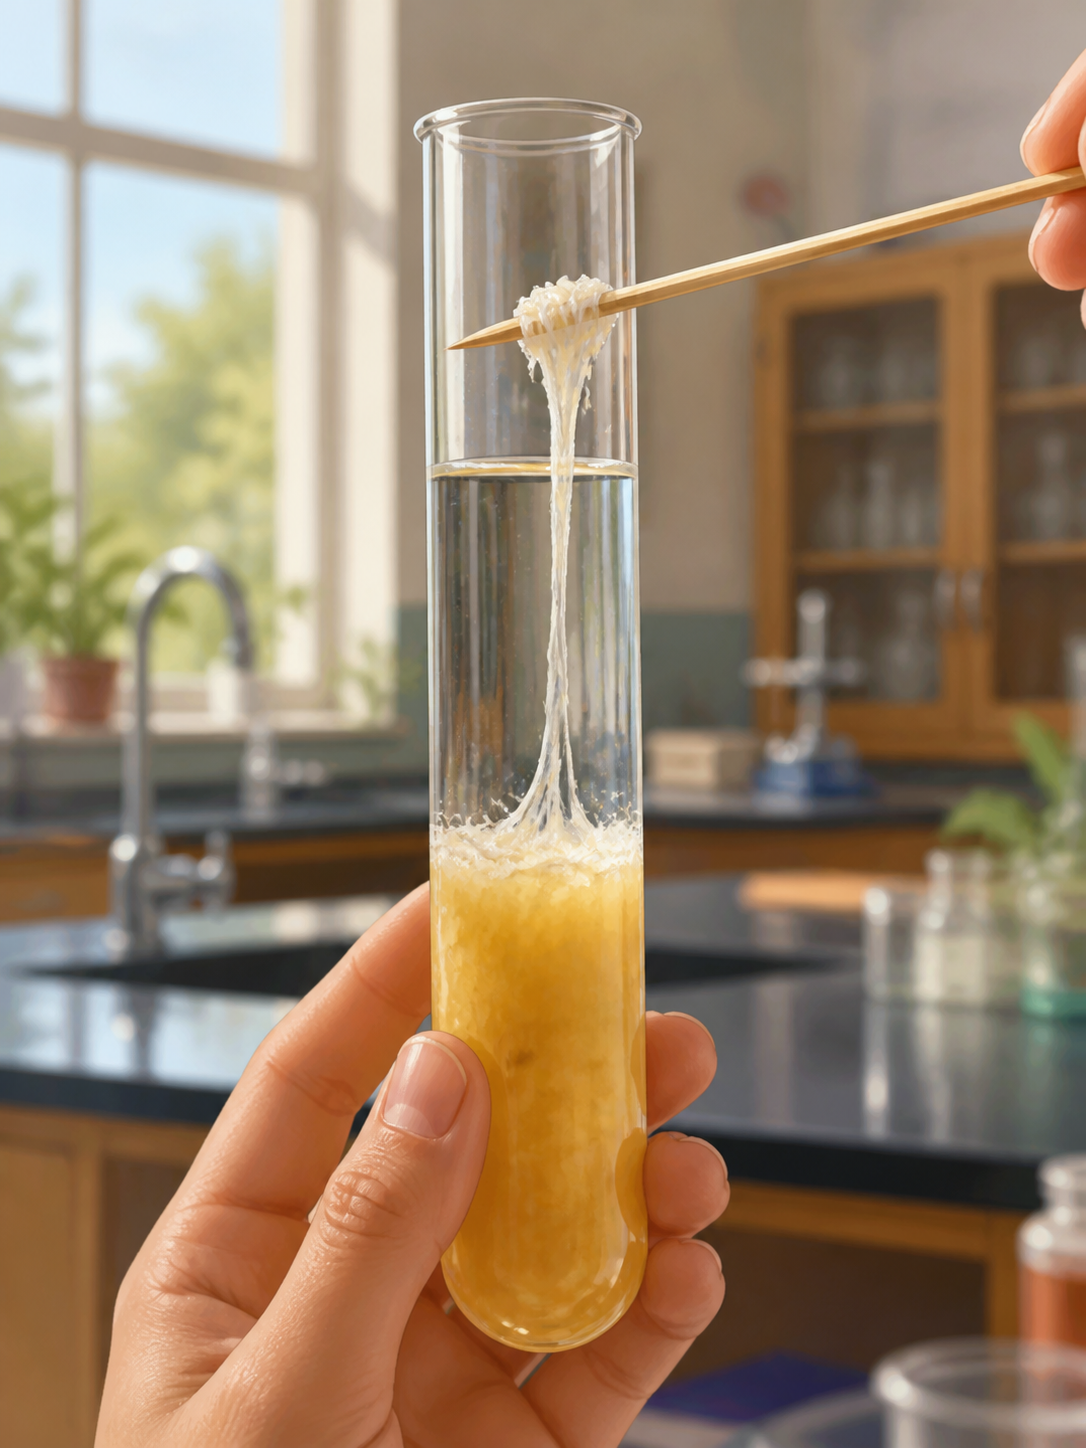
\includegraphics[width=0.42\linewidth]{images/book1/ai/g9-dna-extraction.png}

{\small Le butin de l'extraction à la cuisine~: la molécule
de l'\omterm{def:g9:heredity-and-traits:heredity}{hérédité}, enroulée sur un bâtonnet.}
\end{omfigure}

\begin{proposition}[Ce que la structure de l'ADN explique]\label{prop:g9:genes-and-dna:explains}
Le double brin n'est pas une décoration --- chacune de ses
propriétés répond à une vieille question~:
\begin{itemize}
  \item la \emph{copie} (les divisions fidèles de
        \cref{prop:g5:first-look-at-cells:growth})~: les
        deux brins se complètent lettre à lettre~; séparés,
        chacun reconstruit donc son partenaire --- une
        échelle devient deux échelles identiques, une par
        \omterm{def:g5:first-look-at-cells:cell}{cellule} fille~;
  \item les \emph{\omterm{def:g9:genes-and-dna:gene}{allèles}}~: les versions d'un \omterm{def:g9:genes-and-dna:gene}{gène} sont de
        petites différences d'orthographe dans la suite ---
        même adresse, lettres changées~;
  \item la \emph{mutation}\index{mutation}~: la copie est
        presque parfaite, non parfaite --- une rare lettre
        mal recopiée crée un \emph{nouvel} \omterm{def:g9:genes-and-dna:gene}{allèle}. Le plus
        souvent neutre, parfois nuisible, à l'occasion
        utile~: la \omterm{prop:g9:genes-and-dna:explains}{mutation} est d'où viennent les
        orthographes neuves, et en fin de compte tous les
        \omterm{def:g9:genes-and-dna:gene}{allèles} --- la nouveauté brute dont
        \cref{ch:g9:how-species-change} aura besoin~;
  \item la \emph{lecture}~: une \omterm{def:g5:first-look-at-cells:cell}{cellule} se sert d'un \omterm{def:g9:genes-and-dna:gene}{gène}
        en lisant sa suite et en construisant la molécule
        de travail correspondante --- et chaque sorte de
        \omterm{def:g5:first-look-at-cells:cell}{cellule} lit sa propre sélection de la bibliothèque~:
        l'énigme de \cref{exo:g9:chromosomes:12}, résolue
        comme promis.
\end{itemize}
\end{proposition}
\admitted

\begin{remark}[Un seul code, toute la vie]\label{rem:g9:genes-and-dna:universal}
Le fait le plus profond vient en dernier~: \emph{tout}
\omterm{def:g6:exploring-our-environment:components}{être vivant} écrit ses \omterm{def:g9:genes-and-dna:gene}{gènes} dans les mêmes lettres d'\omterm{def:g9:genes-and-dna:dna}{ADN} et
les lit avec le même code --- le chêne, la \omterm{ex:g6:producing-our-food:bread}{levure}, la
baleine, les \omterm{def:g6:producing-our-food:fermentation}{microbes} de
\cref{ch:g6:producing-our-food}, toi. C'est l'\omterm{prop:g5:first-look-at-cells:principle}{unité du
vivant} (\cref{prop:g5:first-look-at-cells:principle}) à son
fondement, et la preuve la plus forte, à ce jour, de
l'\omterm{def:g6:classification-kinship:tree}{arbre de parenté}
(\cref{rem:g6:classification-kinship:implies})~: une langue
partagée plaide pour une origine partagée. C'est aussi
pourquoi le génie génétique fonctionne --- un \omterm{def:g9:genes-and-dna:gene}{gène} déplacé
d'une \omterm{def:g5:biodiversity:species}{espèce} à une autre reste lisible, comme une phrase
photocopiée dans un autre livre.
\end{remark}

\begin{method}[La lecture à trois niveaux]\label{met:g9:genes-and-dna:levels}
Toute question d'\omterm{def:g9:heredity-and-traits:heredity}{hérédité} se lit désormais à trois niveaux
--- exerce-toi à passer de l'un à l'autre~:
\begin{enumerate}
  \item le \emph{niveau familial}~: qui montre, qui porte,
        qui transmet (\cref{ch:g9:heredity-and-traits})~;
  \item le \emph{niveau chromosomique}~: quels fils, réduits
        de moitié puis rétablis, portent la distribution
        (\cref{ch:g9:chromosomes})~;
  \item le \emph{niveau moléculaire}~: quel \omterm{def:g9:genes-and-dna:gene}{gène}, quels
        \omterm{def:g9:genes-and-dna:gene}{allèles}, quelle orthographe --- et, pour un
        \omterm{def:g9:heredity-and-traits:traits}{caractère} nouveau, quelle \omterm{prop:g9:genes-and-dna:explains}{mutation}.
\end{enumerate}
Une seule histoire, trois grossissements~; une réponse est
complète quand elle tourne aux trois.
\end{method}

\section{Exercices}

\begin{exercise}[$\star$]\label{exo:g9:genes-and-dna:1}
Définis \omterm{def:g9:genes-and-dna:gene}{gène} et \omterm{def:g9:genes-and-dna:gene}{allèle}, avec l'exemple des groupes sanguins.
\end{exercise}

\begin{exercise}[$\star$]\label{exo:g9:genes-and-dna:2}
Pourquoi tout \omterm{def:g9:genes-and-dna:gene}{gène} existe-t-il en deux exemplaires, et où
se tiennent-ils~?
\end{exercise}

\begin{exercise}[$\star$]\label{exo:g9:genes-and-dna:3}
Qu'est-ce que l'information de l'\omterm{def:g9:genes-and-dna:dna}{ADN}, physiquement~?
Combien de lettres, de combien de sortes, dans un jeu
humain~?
\end{exercise}

\begin{exercise}[$\star$]\label{exo:g9:genes-and-dna:4}
Comment le double brin rend-il possible une copie fidèle~?
\end{exercise}

\begin{exercise}[$\star$]\label{exo:g9:genes-and-dna:5}
Qu'est-ce qu'une \omterm{prop:g9:genes-and-dna:explains}{mutation}, et quels sont ses trois
\omterm{def:g9:heredity-and-traits:traits}{caractères} possibles~?
\end{exercise}

\begin{exercise}[$\star$]\label{exo:g9:genes-and-dna:6}
Énonce le fait de \cref{rem:g9:genes-and-dna:universal} et
ses deux conséquences.
\end{exercise}

\begin{exercise}[$\star\star$]\label{exo:g9:genes-and-dna:7}
Mécanise l'enfant aux \omterm{def:g1:the-five-senses:sense}{yeux} bleus de parents aux \omterm{def:g1:the-five-senses:sense}{yeux}
bruns~: les exemplaires, les distributions, et le un sur
quatre.
\end{exercise}

\begin{exercise}[$\star\star$]\label{exo:g9:genes-and-dna:8}
Travaille \cref{ex:g9:genes-and-dna:bloodgroups}~: donne
les couples d'\omterm{def:g9:genes-and-dna:gene}{allèles} derrière chacun des quatre groupes.
\end{exercise}

\begin{exercise}[$\star\star$]\label{exo:g9:genes-and-dna:9}
Résous \cref{exo:g9:chromosomes:12} dans les termes de ce
chapitre~: que lit un \omterm{def:g8:nervous-communication:neuron}{neurone} que ne lit pas une \omterm{def:g5:first-look-at-cells:cell}{cellule} de
\omterm{def:g1:the-five-senses:sense}{peau}~?
\end{exercise}

\begin{exercise}[$\star\star$]\label{exo:g9:genes-and-dna:10}
Décris l'extraction à la cuisine et dis ce que fait chaque
ingrédient de cuisine.
\end{exercise}

\begin{exercise}[$\star\star$]\label{exo:g9:genes-and-dna:11}
Applique les trois niveaux de
\cref{met:g9:genes-and-dna:levels} au menton de la chapelle
de \cref{pb:g9:heredity-and-traits:1}.
\end{exercise}

\begin{exercise}[$\star\star\star$]\label{exo:g9:genes-and-dna:12}
«~La \omterm{prop:g9:genes-and-dna:explains}{mutation} écrit, le brassage distribue, l'expression
montre.~» Attribue à chaque verbe son mécanisme et son
chapitre --- et dis lequel des trois crée des orthographes
vraiment \emph{neuves}.
\end{exercise}

\section{Problème~: la photocopieuse en panne}

\begin{problem}[{Problème du week-end --- un gène suivi de
l'orthographe à l'arbre généalogique}]\label{pb:g9:genes-and-dna:1}
Suis un cas (inventé mais typique)~: un \omterm{def:g9:genes-and-dna:gene}{gène} de pigment
dont l'\omterm{def:g9:genes-and-dna:gene}{allèle} fonctionnel, P, construit un pigment de la
\omterm{def:g1:the-five-senses:sense}{peau} et des cheveux~; il y a longtemps, une erreur de copie
a créé l'\omterm{def:g9:genes-and-dna:gene}{allèle} cassé p --- mal orthographié au point
d'être illisible, ne construisant rien. Les porteurs de P
avec p ont l'air ordinaires~; un enfant qui reçoit p et p
ne construit aucun pigment --- des cheveux et une \omterm{def:g1:the-five-senses:sense}{peau} très
clairs, des \omterm{def:g1:the-five-senses:sense}{yeux} fragiles au soleil (l'état existe chez
beaucoup d'\omterm{def:g5:biodiversity:species}{espèces}).

\medskip\noindent\textbf{Partie I --- Niveau moléculaire.}
\begin{enumerate}
  \item Nomme l'origine de p, d'après
        \cref{prop:g9:genes-and-dna:explains} --- que
        s'est-il physiquement passé, une fois, dans la
        lignée reproductrice d'un ancêtre~?
  \item Pourquoi P avec p a-t-il l'air ordinaire~? Quel mot
        de vocabulaire décrit le voyage de p~?
  \item Pourquoi p avec p change-t-il la construction~?
        Qu'est-ce qui manque, et de quelle sorte de
        machinerie, au sens de
        \cref{def:g9:genes-and-dna:gene}~?
  \item L'état apparaît chez beaucoup d'\omterm{def:g5:biodiversity:species}{espèces}. Que
        prédit \cref{rem:g9:genes-and-dna:universal} sur
        l'orthographe de leurs \omterm{def:g9:genes-and-dna:gene}{gènes} de pigment~?
\end{enumerate}

\medskip\noindent\textbf{Partie II --- Niveaux
chromosomique et familial.}
\begin{enumerate}[resume]
  \item Deux parents porteurs (P avec p chacun)~: donne les
        quatre distributions également probables pour un
        enfant, et la probabilité de la construction p avec
        p.
  \item Leur fille p avec p naît de deux parents d'aspect
        ordinaire. Quel mystère de l'album
        (\cref{ex:g9:heredity-and-traits:skip}) vient de se
        jouer, mécanisme complet~?
  \item Les enfants de cette fille avec un partenaire P
        avec P~: que portent-ils tous, et que ne montre
        aucun d'eux~?
  \item Suis les véhicules de l'\omterm{def:g9:genes-and-dna:gene}{allèle} sur une
        transmission~: le voyage de p de la grand-mère au
        petit-enfant, fil après fil et \omterm{def:g8:sexual-reproduction:gametes}{gamète} après \omterm{def:g8:sexual-reproduction:gametes}{gamète}.
\end{enumerate}

\medskip\noindent\textbf{Partie III --- Le compte rendu à
trois niveaux.}
\begin{enumerate}[resume]
  \item Écris le cas aux trois niveaux de
        \cref{met:g9:genes-and-dna:levels}, une phrase pour
        chacun.
  \item Un camarade demande pourquoi l'orthographe cassée
        n'a pas simplement été «~réparée~» il y a
        longtemps. Réponds par l'aspect ordinaire du
        porteur --- où p se cache-t-il de tout jugement sur
        ses effets~?
  \item La protection solaire compte davantage pour la
        fille que pour ses parents porteurs. Relie le
        \omterm{def:g9:heredity-and-traits:traits}{caractère}, le couple d'\omterm{def:g9:genes-and-dna:gene}{allèles} et le milieu en une
        phrase (le tissage de
        \cref{prop:g9:heredity-and-traits:sorting}).
  \item Termine par l'image de la photocopieuse rendue
        exacte~: ce qui copie, ce qui a été mal copié une
        fois, et pourquoi l'erreur est maintenant copiée
        fidèlement.
\end{enumerate}
\end{problem}
